\section{Introduction}\label{sec:introduction}
    \todo[inline]{Here goes short introduction with mention that this is a work about \acf{tool}}

\subsection{Scope}
    The thesis covers the process of development of the toolbox for rapid prototyping of satellite's control systems. \autoref{sec:introduction} describes the aim of this work and discusses the topic of prototyping tools. \autoref{sec:toolbox} goes into detail about the architecture of \ac{tool}, its features and methods of implementation. Also here there are described the ways of connecting \ac{tool} with various visualization tools. \autoref{sec:documentation} explains the documentation and usage of \ac{tool}, while in \autoref{sec:examples} there are examples showing how the toolbox can be used in real life applications. Finally, \autoref{sec:conclusions} discusses the conclusions from the development process and the possibilities for improvements of \ac{tool}.

\subsection{Aim}
    The process of effective space-related project management, from the conception of the idea, through production, to disposal, features high costs and often various unpredictable risks. Due to this, a project life cycle is usually divided into distinct phases, allowing for introduction of conducting product reviews within rigid timeframes. An example of such a workflow, adopted by most major agencies such as ESA\cite{managementecss} and NASA\cite{kapurch2010nasa}, is a division of the project life cycle into phases, as it can be seen on \autoref{fig:phases}. While the design of a project is often an iterative process, the phases and reviews that conclude them exist as a checkpoints, after which the design of the project is to be unchanged, on a level of details progressing as phases do. For example, as one can see, Phase B is usually ended by the \ac{pdr}. In the case of a spacecraft, for the \ac{pdr}, a major architecture parameters have to be defined, such as volume and weight ramifications, top-level designs of solutions for major requirements have to be presented - for a practical example: for high-resolution Earth observation mission the type of the actuators which fulfills precision requirements has to be chosen.

    \begin{figure}[H]
        \centering
        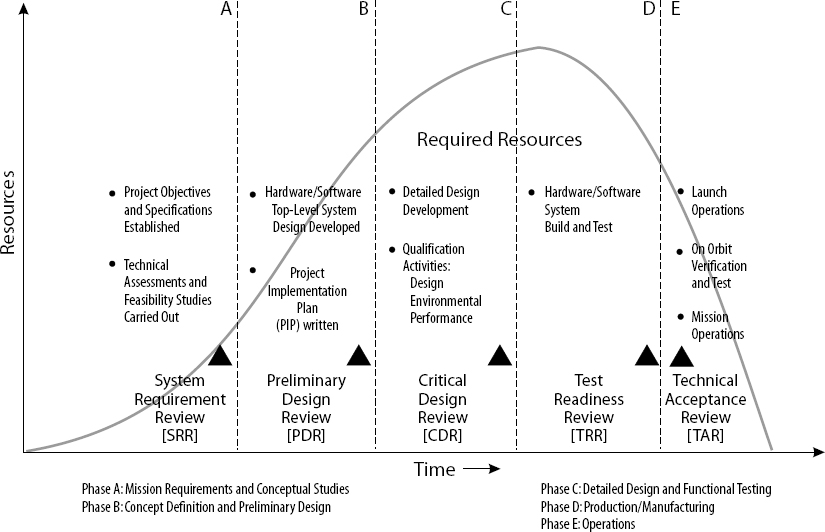
\includegraphics[width=1\textwidth]{1-introduction/phases}
        \caption{Typical space project phases and its life cycle\cite{nguyen2000effective}}
        \label{fig:phases}
    \end{figure}

    The aim of this thesis work is to build and provide a ready to use open source product - a toolbox for small and low budget satellite projects.  The toolbox features allow for a initial design of spacecraft's \ac{adcs}, which means that they allow for, i.a. simulation of spacecraft orbit, testing the feasibility of various actuation methods and testing the effectiveness of different control algorithms in given use cases. \todo{refine the list of examples this} That software would then allow smaller and inexperienced teams of spacecraft designers to better prepare for design milestones like \ac{pdr}, when there is not enough time to create a full simulation of their spacecraft \ac{adcs} subsystems.\todo{also, add some lines about how it can be used for learning in general (like some university courses)}
    \\
    \todo[inline]{While the toolbox is by itself a tool for practial use, the thesis also serves as as a review of available solutions, so it can be used by future control engineers as a learning material.}

    Furthermore, the objectives of the toolbox itself are described in Chapter \ref{toolbox:objectives}.

    % find how to ref by full name

    \todo[inline]{put here an example from my experience with BEXUS}

\subsection{Prototyping tools}
\todo[inline]{refer to CAE software}

\subsection{Small spacecraft simulations}

\subsection{Already existing tools}
    ... This is to show that, while the toolbox for \ac{adcs} prototyping or development is not an innovative idea, but since some existing solutions are not best fit for the job of rapid prototyping and others are unavailable or paid, there is a need for a new, open-source one.
    
    \todo{Should I put "advantages" and "disadvantages" here at the end of every point?}

    \subsubsection{MATLAB CubeSat Simulation Library}
        \todo{how to write that it was considered to expand this rather than develop own toolbox}
        CubeSat Simulation Library is a part of Aerospace Blocks created by MathWorks Aerospace Products Team. Using it one can model motion and dynamics of CubeSats and nano satellites. It provides the most basic features, like the simulation of pre-set attitude scenarios, basic actuators and sensors models and integration with MATLAB's Virtual World visualization tools.
        
        \begin{figure}[H]
            \centering
            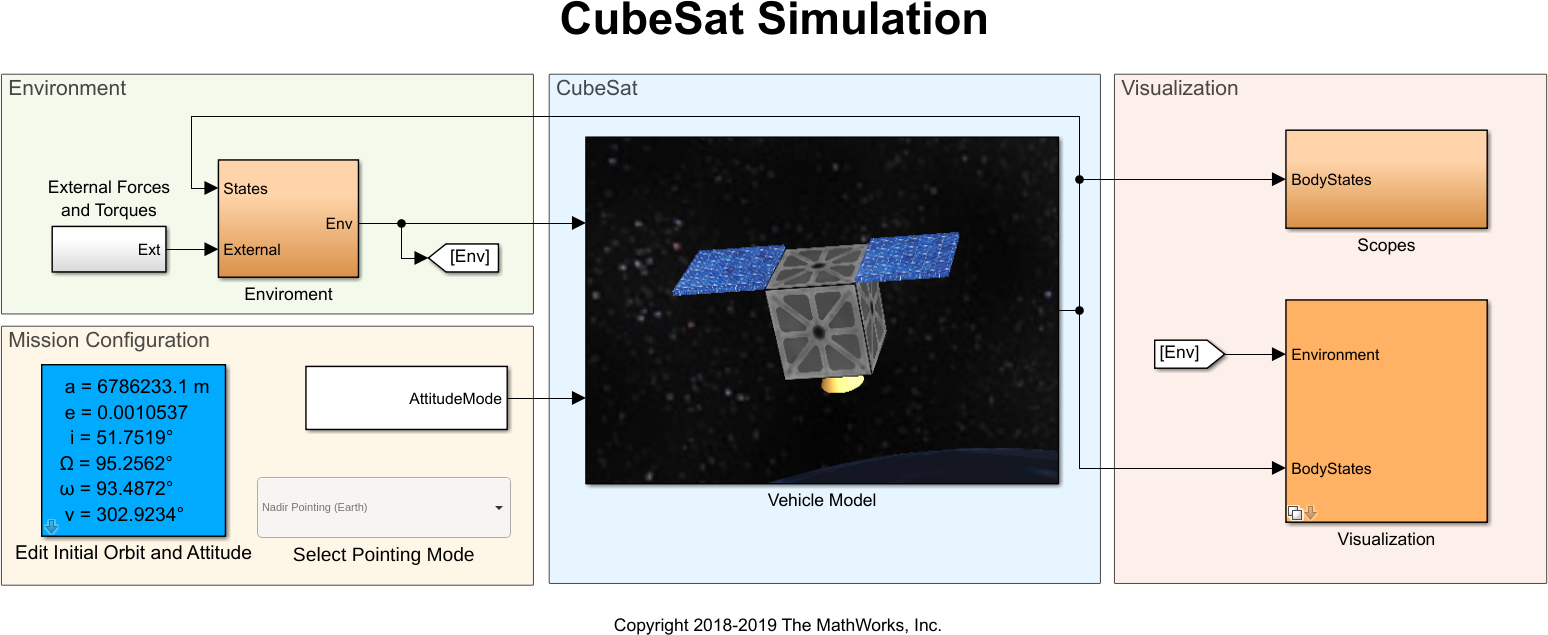
\includegraphics[width=1\textwidth]{1-introduction/matlab_cubesat}
            \caption{Top-level view of the example project of the MATLAB CubeSat Simulation Library}
            \label{fig:matlab_cubesat}
        \end{figure}

        This library, while conceptually most similar to the \ac{tool}, it lacks some functionalities. For example, for actuators, it provides only general models for perfect and second-order actuators. In \ac{tool}, the actuators are full models, which allows not only for reducing the number of layers of abstraction between the user and the simulation, but also for things like calculation of energy expended by the actuator. Also, this toolbox is sparsely documented - while most functionalities are described within their Simulink block masks, there is no comprehensive guide about how to use them in own models.
        % \cite{matlabcubesat}
        \todo{does this explanation belong here?}

    \subsubsection{PrincetonSATELLITE Spacecraft Control Toolbox}
        PrincetonSATELLITE Spacecraft Control Toolbox is a commercial solution for building spacecraft Simulations. I contains over two thousand functions for attitude and orbit dynamics, simulation, estimation, analysis and design. This is the most robust and comprehensive toolbox available, includes online API, well written documentation and additional modules for unique applications like formation flying, fusion propulsion or solar sails. Yet this is a paid solution and even the cheapest option - CubeSat Edition - may be out of price range for smaller teams.

    \subsubsection{PROPAT Toolbox}
        PROPAT is is a small set of functions in Matlab to simulate and propagate orbit and attitude of an Earth's satellite, developed by the single person as an open-source toolbox. Several functions allow to transform between orbit and attitude coordinates and for propagation or rigid body attitude. PROPAT contains only MATLAB scripts, which while useful and can be used as a part of the simulation, do not combine into a model of a whole spacecraft's \ac{adcs} subsystem.

    \subsubsection{GAST Toolbox}
        \begin{figure}[H]
            \centering
            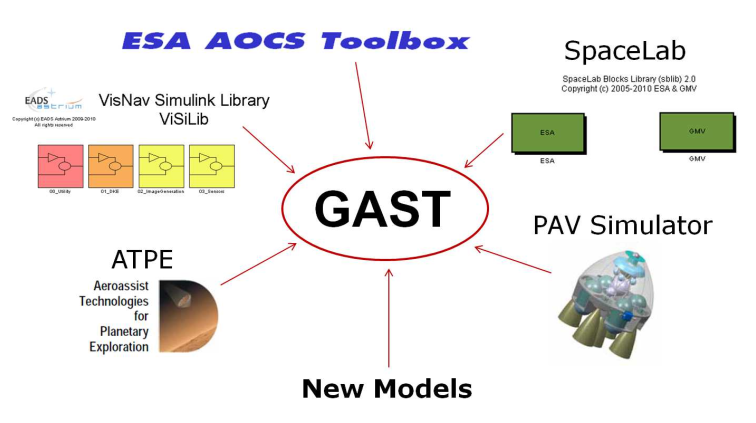
\includegraphics[width=1\textwidth]{1-introduction/gast}
            \caption{Representation of the consolidation of TEC-ECN toolboxes}
            \label{fig:gast}
        \end{figure}

        The GAST toolbox is the result of the consolidation of several toolboxes available in \ac{tec} of \ac{estec}, such as the old AOCS Toolbox, the SpaceLAB library, the ViSiLib library, the ATPE simulator, and the PAV simulator. In addition to consolidating these toolboxes, new models were developed for the GAST toolbox according to the needs of the section. \autoref{fig:gast} shows a pictorial representation of the consolidation of the toolboxes of TEC-ECN. This software was developed in \ac{tec} in 2008, but since it is a product of \ac{esa}, it is not available for use for wider audience.

    \subsection{Modules available on MathWorks MATLABCentral}
    \todo[inline]{describe these modules in two sentences}
    \subsubsection{SAT-LAB}
    \todo[inline]{https://www.mathworks.com/matlabcentral/fileexchange/63344-sat-lab-a-matlab-graphical-user-interface-for-simulating-and-visualizing-keplerian-satellite-orbits}
    \subsubsection{Satellite Orbit Modeling}
    \todo[inline]{https://www.mathworks.com/matlabcentral/fileexchange/54877-satellite-orbit-modeling}
    \subsubsection{Satellite Orbits: Models, Methods and Applications}
    \todo[inline]{https://www.mathworks.com/matlabcentral/fileexchange/54840-satellite-orbits-models-methods-and-applications}
    \subsubsection{Smart Nanosatellite Attitude Propagator (SNAP) }
    \todo[inline]{https://www.mathworks.com/matlabcentral/fileexchange/68652-smart-nanosatellite-attitude-propagator-snap}
    

\todo[inline]{Also, write somewhere that while the Toolboxes/Simulations like these are present within papers online, they are nowehere to be found to download and it is hard and time-consuming to recreate them from papers.}
